Ein wesentlicher Aspekt der K.I.\ ist es die aktuelle Spielfeldsituation der unterschiedlichen Spieler zu bewerten.
Dadurch ist es der K.I.\ m\"oglich Spielz\"uge besser einzustufen und gegebenenfalls das Spiel mit Spezialsteinen zu beeinflussen.
Ein naiver Ansatz w\"are der Vergleich der aktuellen Spielsteine jeden Spielers.
Dieses Vorgehen reicht jedoch nicht f\"ur eine ad\"aquate Bewertung der Spielsituation.
In Abbildung 1 w\"urde die naive Vorgehensweise den roten Spieler besser einstufen, jedoch hat er hier keinerlei m\"ogliche Spielz\"uge.
Der rote Spieler kann trotz dieser \"Uberlegenheit nicht mehr gewinnen, da der blaue Spieler im n\"achsten Spielzug \"uber alle roten hinweg ziehen kann.
Genau aus diesem Grund reicht eine naive Spielfeldbestimmung nicht f\"ur ein aussagekr\"afigtes Resultat aus.

\vspace{1em}
\begin{minipage}{\linewidth}
    \centering
    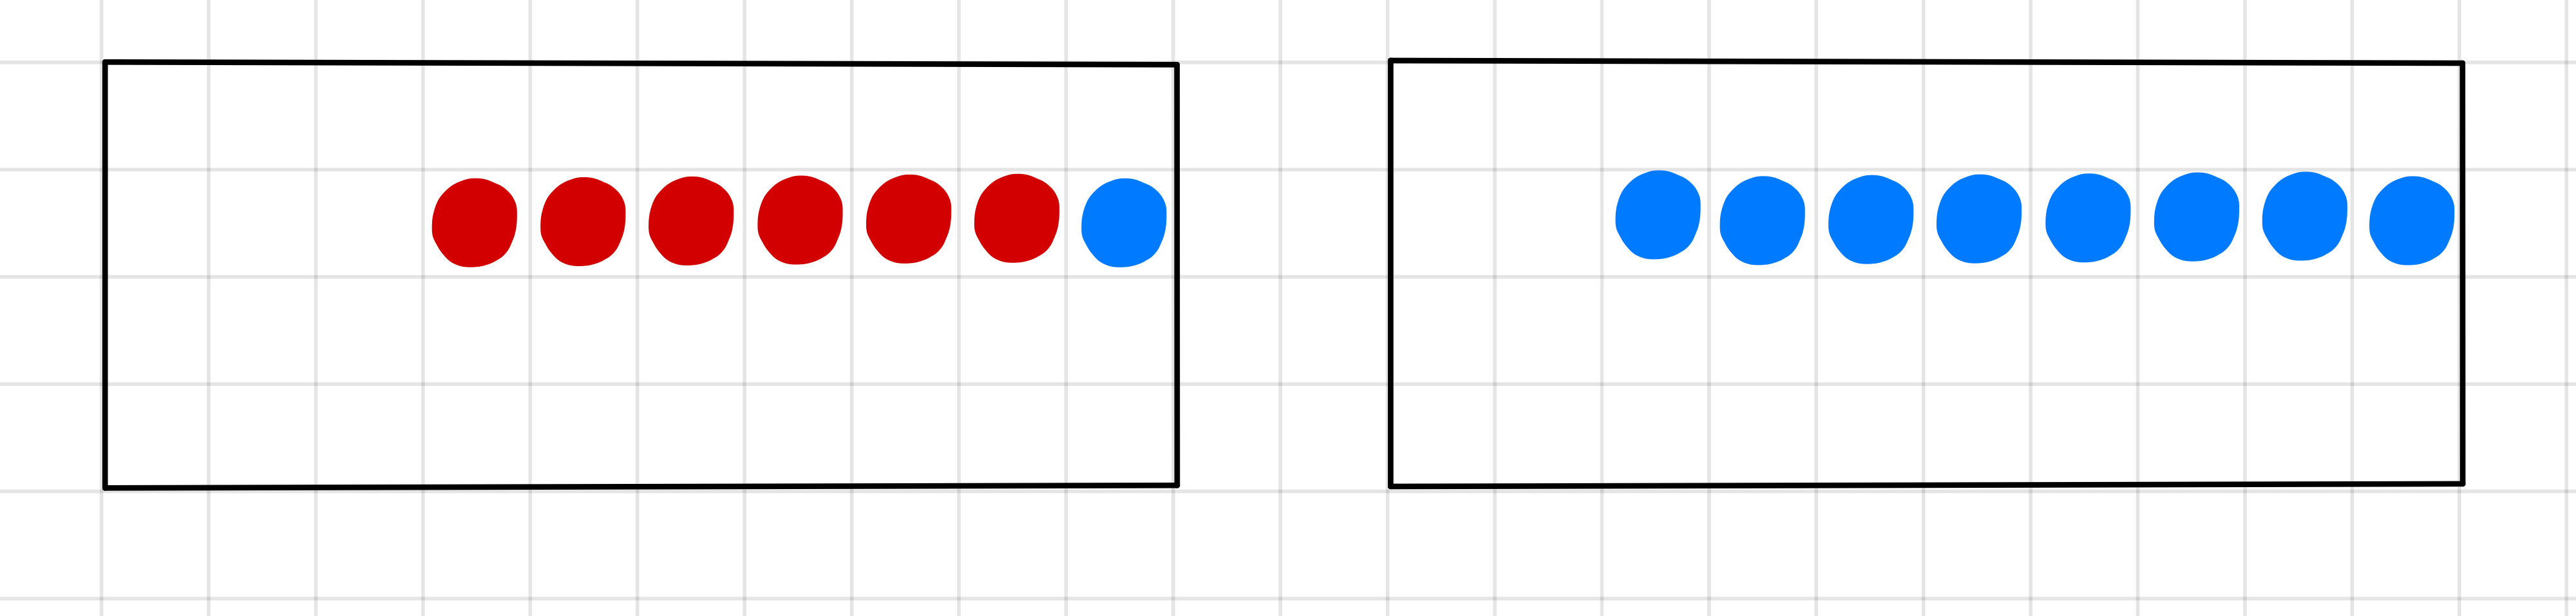
\includegraphics[width=0.6\linewidth]{pics/naive-spielsituation}
    \captionof{figure}[Spielfeldsituation 01]{Problematik der naiven Bewertung}
    \label{fig:naivespielfeld01}
\end{minipage}

\subsection{Bestandteile und Implementierung}\label{subsec:bestandteile-und-implementierung}

\subsubsection{Variante 1: Gewichtung der einzelnen Felder}
Wie bereits in der Einleitung gezeigt ist das Abz\"ahlen der Spielsteine nicht ausreichend.
Eine bessere Alternative ist es das Spielfeld an sich zu bewerten.
Es gibt gewisse Positionen die f\"ur einen Spieler wertvoller sind als andere.
Zu diesen Positionen z\"ahlen unter anderem Kanten und Ecken, da es wesentlich schwieriger, bis garnicht m\"oglich ist, diese einzunehmen.
Eine Au"snahme stellt hier das Einnehmen mithilfe von \"Uberschreib-, bzw.\ Spezialsteine dar.
Insbesondere sind Felder die zwei Felder oder mehr von einem Bonusfeld in direkter Richtung entfernt sind h\"oher gewichtet, da sie die M\"oglichkeit geben einen solchen Bonusstein einzunehmen, falls ein Gegner auf ein direktes Nachbarfeld des Spezialfeldes zieht.

\vspace{1em}
\begin{minipage}{\linewidth}
    \centering
    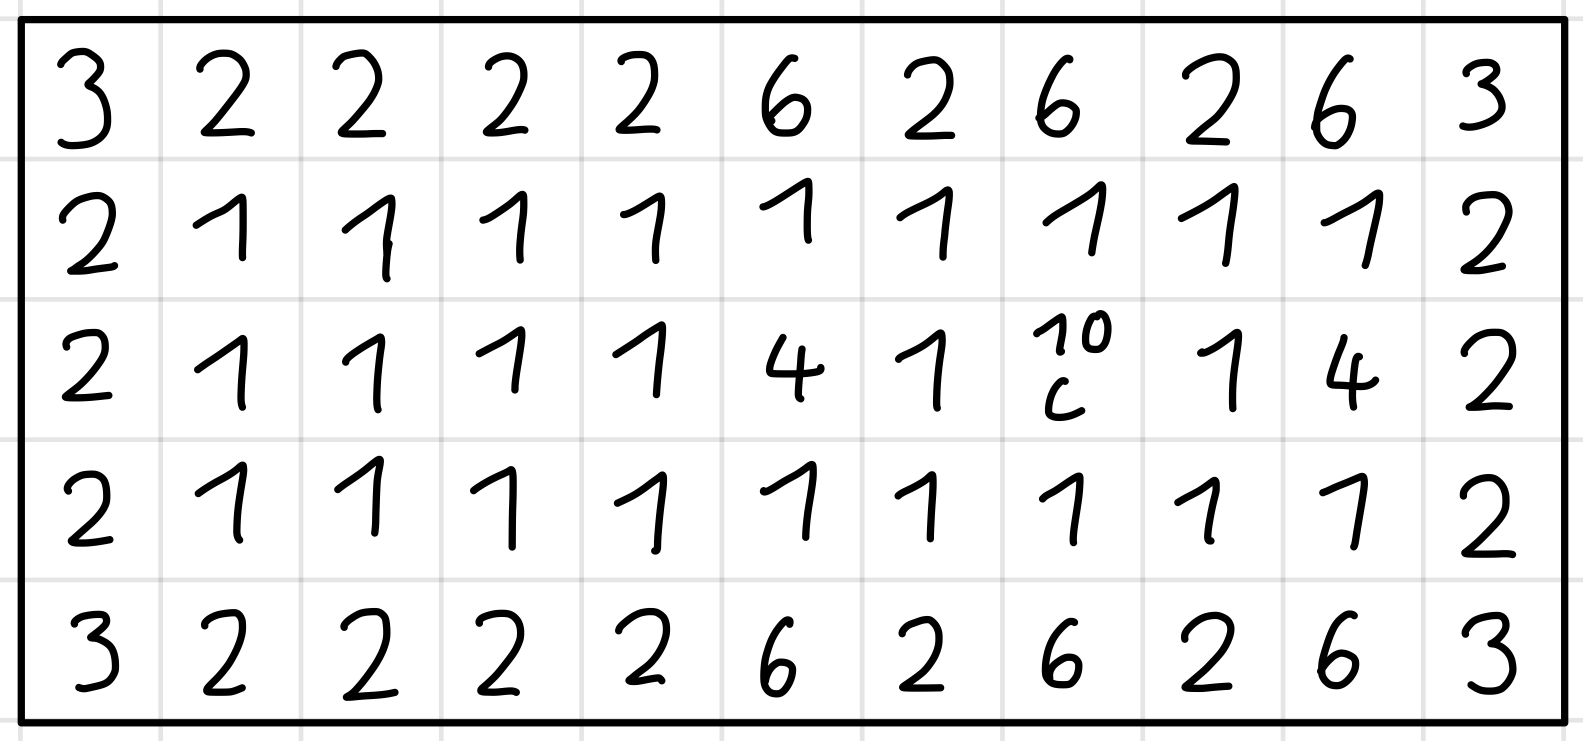
\includegraphics[width=0.5\linewidth]{pics/bewertung}
    \captionof{figure}[Bewertungsverfahren 01]{Spielfeldpositionen mit Gewichtungen}
    \label{fig:bewertungsverfahren01}
\end{minipage}

Der Score eines Spielers setzt sich dann aus der Summe der belegten Felder mit der entsprechenden Gewichtung.

Dieses Bewertungsverfahren bietet Vor- und Nachteile.
Positiv ist es, dass bei Beginn des Spieles jedem Feld eine Gewichtung zugeteilt wird und diese nur noch durch erreichen von Spezialfeldern geringf\"ugig ge\"andert wird.
Negativ ist jedoch, dass dieses Bewertungsverfahren besonders bei gro"sen rechteckigen Spielfeldern mit wenig Spezialfeldern ann\"ahernd wie die naive Variante funktionert.

\subsubsection{Variante 2: Aussage über die möglichen Spielzüge}
Eine andere Vorgehensweise ist es, Spielsituationen anhand der Beweglichkeit der Spieler einzustufen.
Hierbei wird die Anzahl an Spielz\"ugen eines jeden Spielers bestimmt und miteinander verglichen.
Wie bereits in der Einleitung gezeigt kann ein Spieler seine positive Stellung nur halten, solange er weiterhin spielf\"ahig bleibt.
Aus diesem Grund wird in diesem Ansatz bestimmt wie beweglich ein Spieler gegen\"uber die Anderen ist.

Ein Vorteil dieses Verfahrens im Gegensatz zur ersten Variante ist es, dass die Form und gr\"o"se des Spielfeldes keine negativen Einfl\"usse auf diesen Alogithmus hat.
Ein Problem daran ist jedoch, dass diese Verfahren bei gro"sen Maps und bei fortschreiten des Spieles extrem rechenlastig und zeitintesiv wird, da es immer mehr Z\"uge vorrausberechnen muss.


\bigskip
\newpage